\documentclass[11pt,a4paper]{article}
\usepackage[margin=2.2cm]{geometry}
\usepackage{graphicx,booktabs,float,amsmath,hyperref}
\usepackage[T1]{fontenc}
\hypersetup{colorlinks=true,linkcolor=blue}
\title{VLSI Design Course Project, Part II\\SIMD-Reconfigurable 8-bit Adder}
\author{Bhargav, 2025102061\\IIIT Hyderabad, Monsoon 2026}
\date{}
\begin{document}
\maketitle
\tableofcontents
\newpage
\section{Task}
Part II builds an 8-bit adder from two instances of the Part I 4-bit carry look-ahead adder, CLA0 for bits 3..0 and CLA1 for bits 7..4, with a control input SIMD\_MODE:
\begin{itemize}
\item \textbf{SIMD\_MODE = 0, 8-bit mode:} the carry-out of CLA0 propagates into the carry-in of CLA1.
\item \textbf{SIMD\_MODE = 1, dual 4-bit mode:} the inter-block carry is forced to 0, so CLA0 and CLA1 add two independent 4-bit numbers.
\end{itemize}
A carry-gating cell between the two blocks does the switching. Its cost is measured against a \textbf{baseline}: the same two adders with CLA0's carry-out wired straight to CLA1's carry-in.

Everything here uses the provided TSMC 180\,nm model in ngspice at 1.8\,V, and MAGIC with the provided SCN6M\_DEEP technology file, $\lambda = 0.09\,\mu$m. Both 4-bit blocks are the final Part I adder with its final transistor sizes. Every output drives a $W_p/W_n = 20\lambda/10\lambda$ inverter, and every input is driven through a shaper and an x2 inverter, as in Part I.


\section{Architecture}

\begin{figure}[H]\centering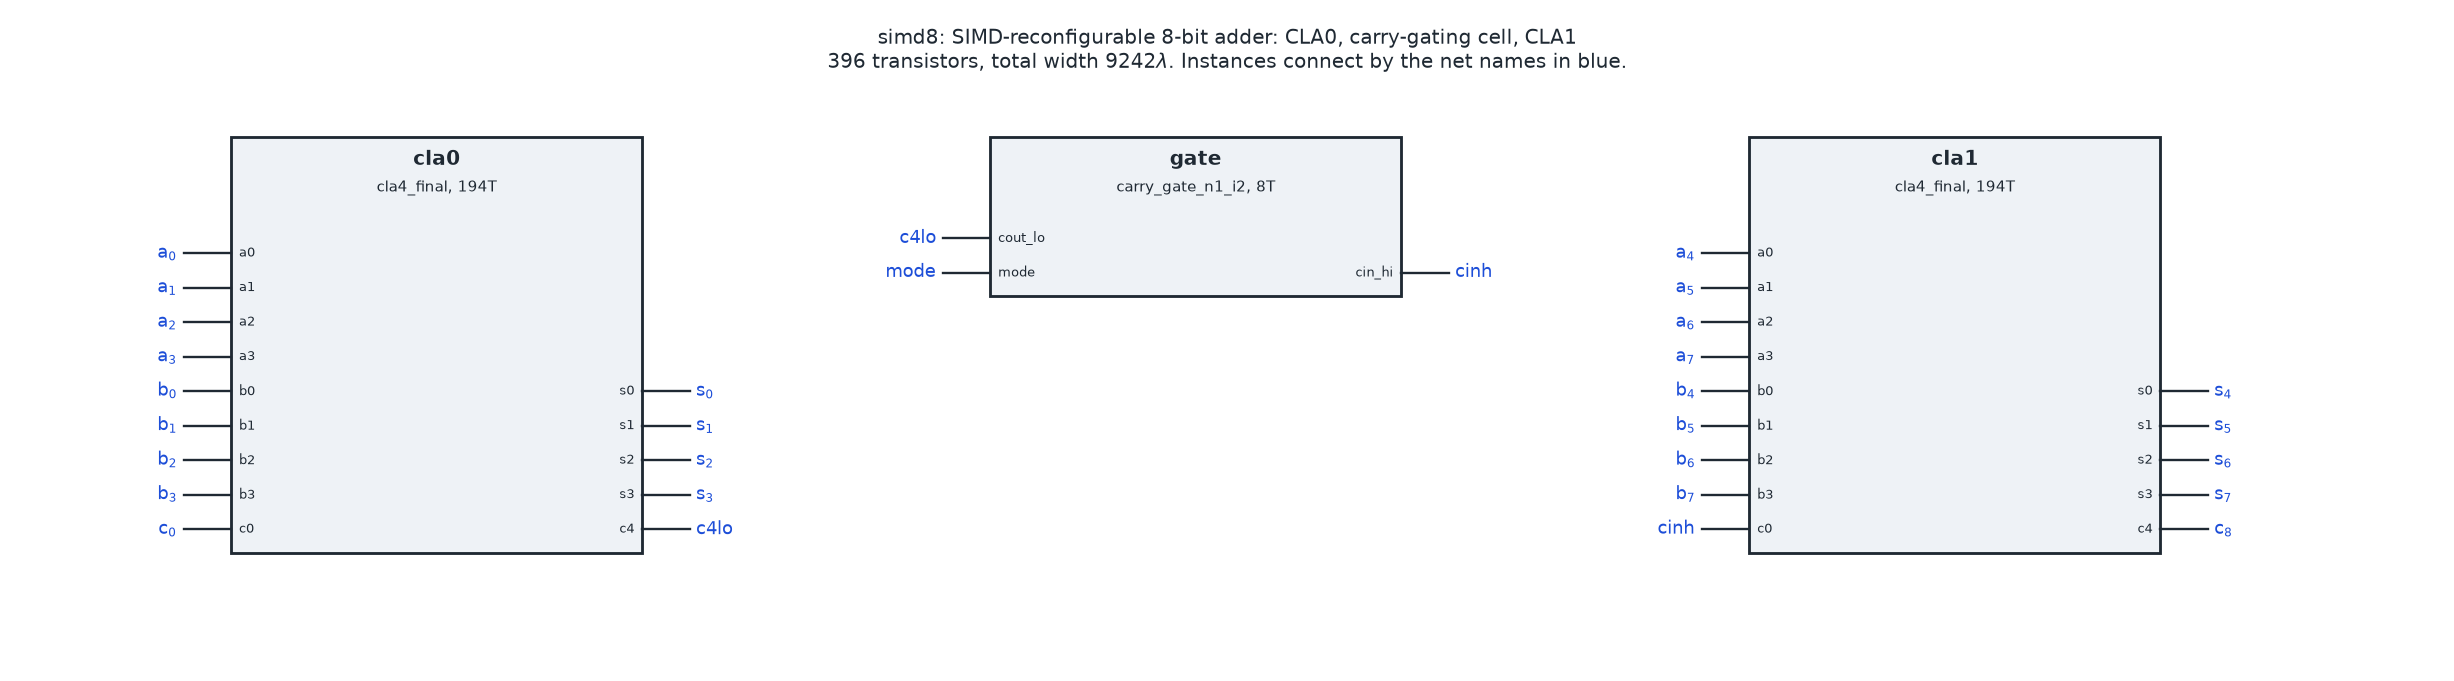
\includegraphics[width=\textwidth]{figures/2.0a_simd8-blocks.png}\caption{SIMD 8-bit adder: CLA0, the carry-gating cell and CLA1. c4lo is CLA0's carry-out, cinh is CLA1's carry-in.}\end{figure}

\begin{figure}[H]\centering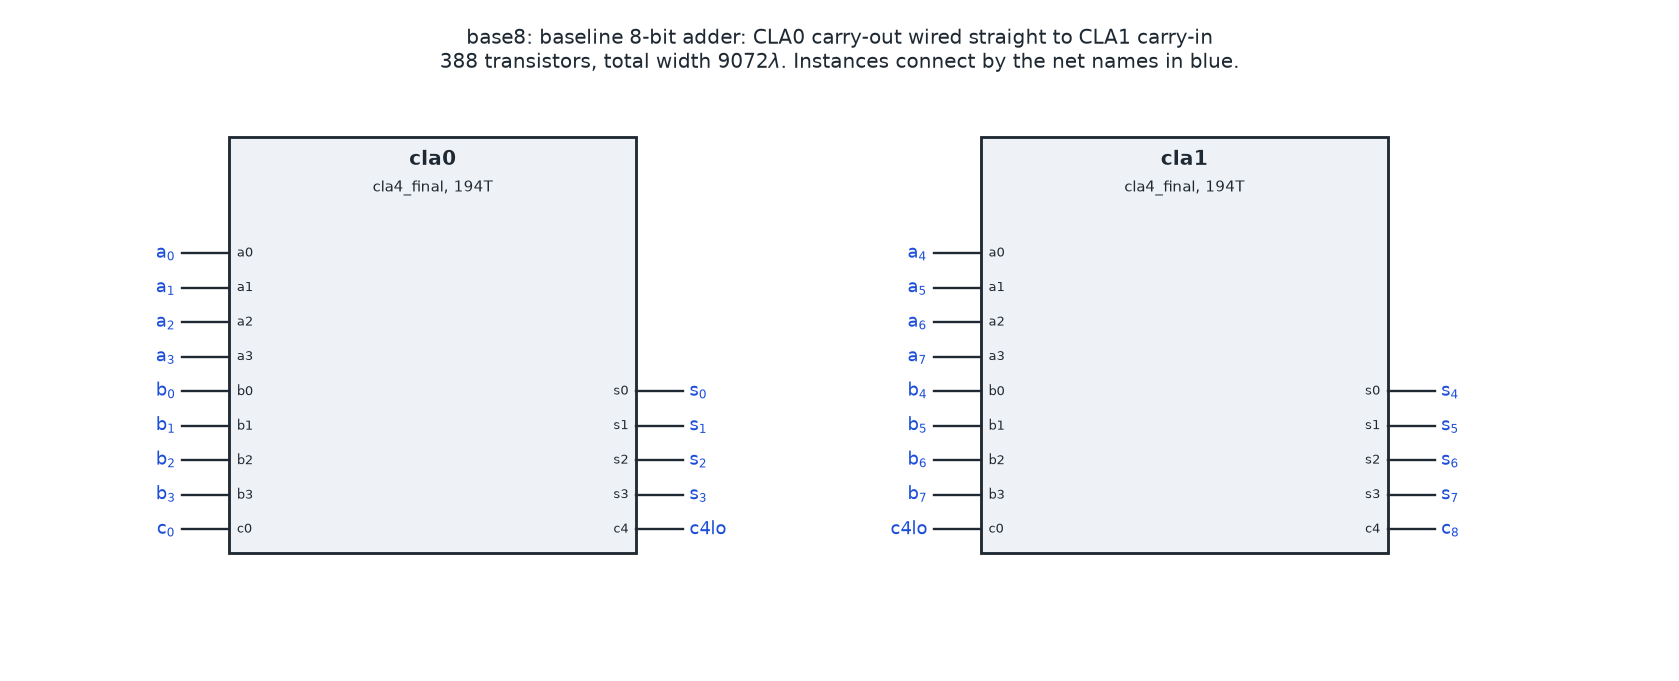
\includegraphics[width=\textwidth]{figures/2.0b_base8-blocks.png}\caption{Baseline 8-bit adder: CLA0's carry-out c4lo goes straight to CLA1's carry-in.}\end{figure}

The SIMD design also brings CLA0's carry-out to an output, c4lo, because in dual mode it is the carry of the lower 4-bit result. It drives the same $20\lambda/10\lambda$ load as the other outputs.

\textbf{Functional check.} Both netlists were evaluated at switch level on 3000 random inputs each, against the behavioural model: 0 errors.


\section{The carry-gating cell}

The carry into CLA1 must equal CLA0's carry-out in mode 0 and be 0 in mode 1:
\[ c_{in,hi} = c_{out,lo} \cdot \overline{\mathrm{SIMD\_MODE}} \]
This is an AND gate. In static CMOS, the cell uses a NAND2 followed by an inverter on the carry path, and a unit inverter for $\overline{\mathrm{SIMD\_MODE}}$. SIMD\_MODE is set before an add and held, so that inverter is off the timing path. Static CMOS was kept for the same reasons as in Part I: full swing and no static current.

\begin{figure}[H]\centering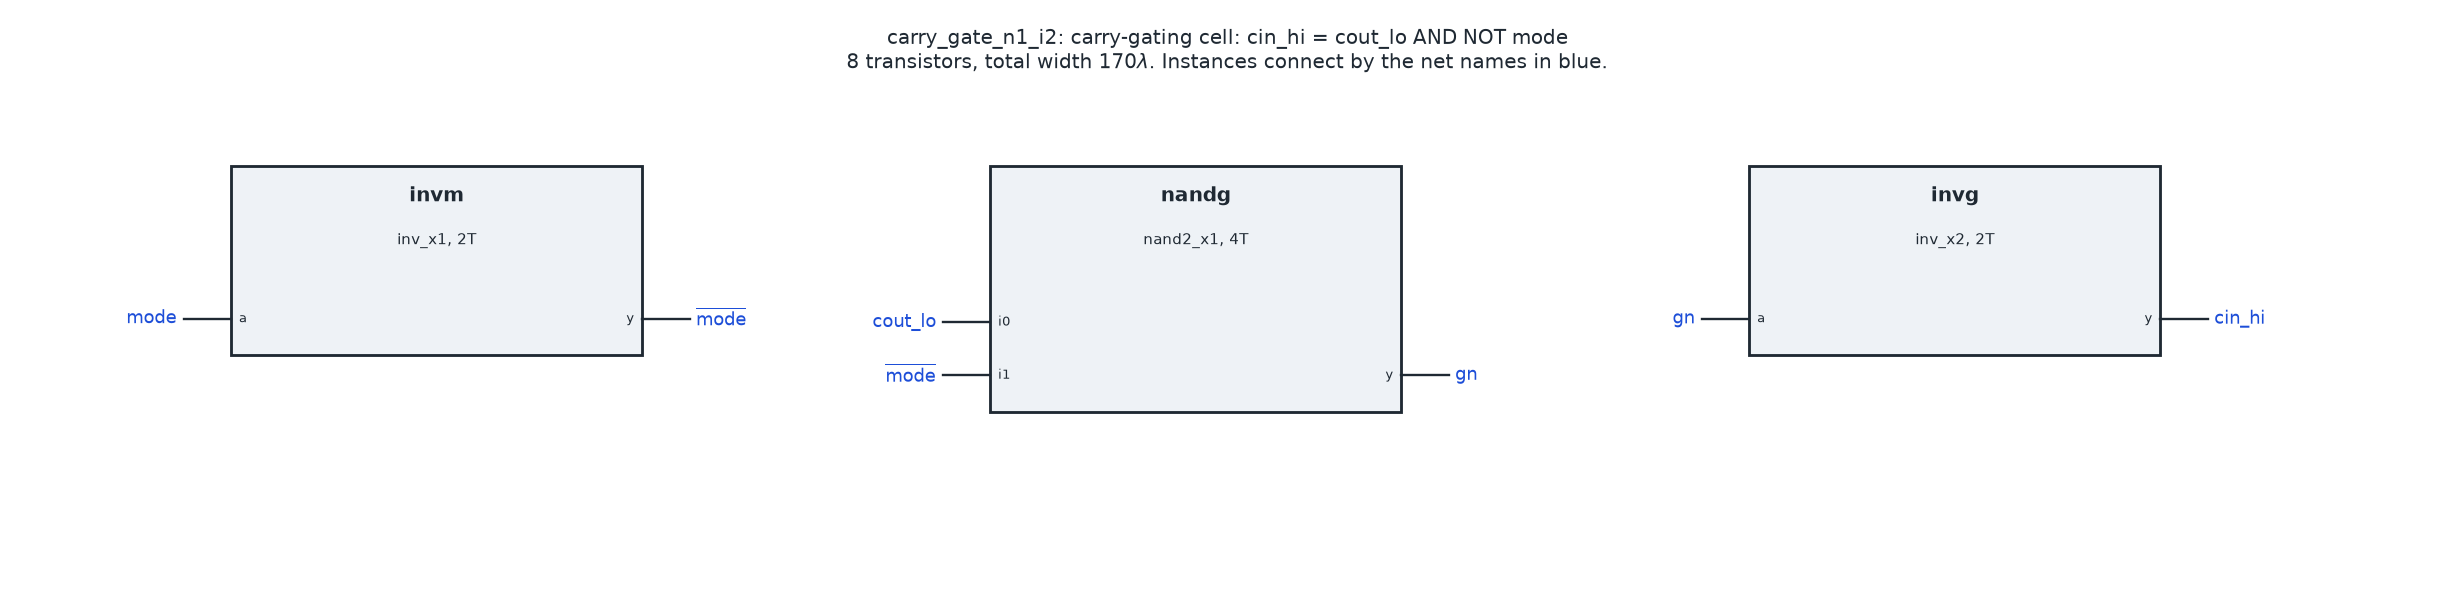
\includegraphics[width=\textwidth]{figures/2.0c_gate-blocks.png}\caption{Carry-gating cell, 8 transistors.}\end{figure}

\begin{figure}[H]\centering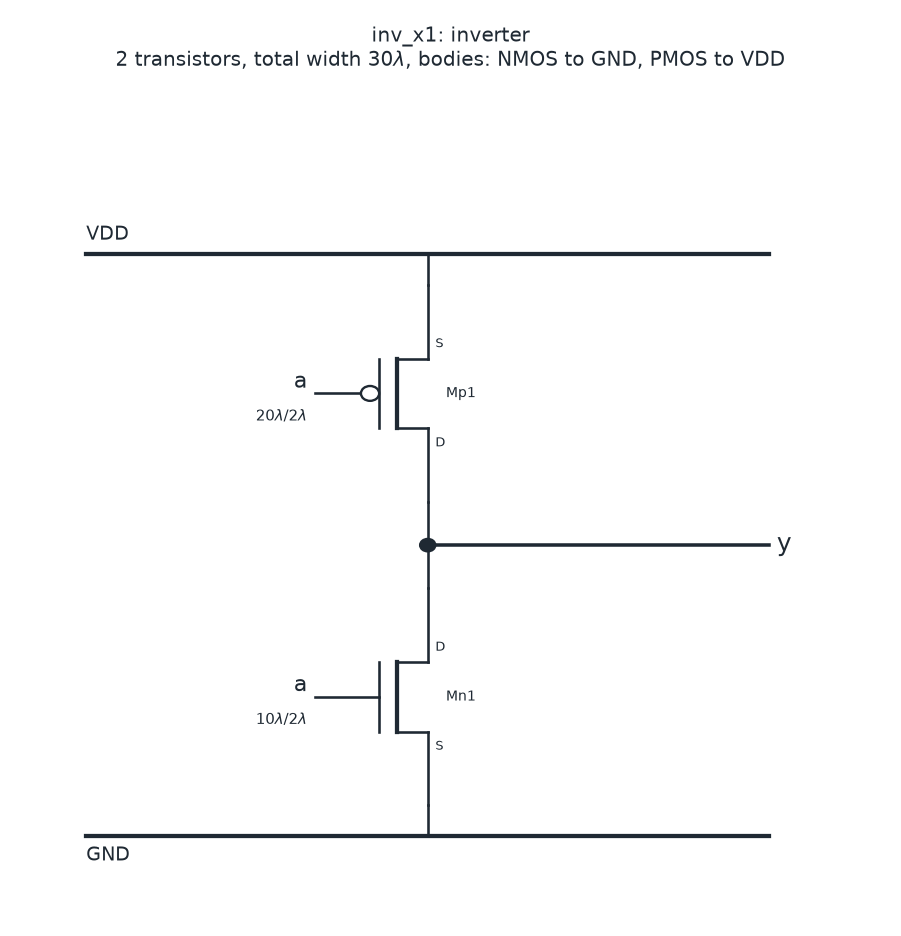
\includegraphics[width=0.32\textwidth]{figures/2.0f_gate-inv-x1.png}\hfill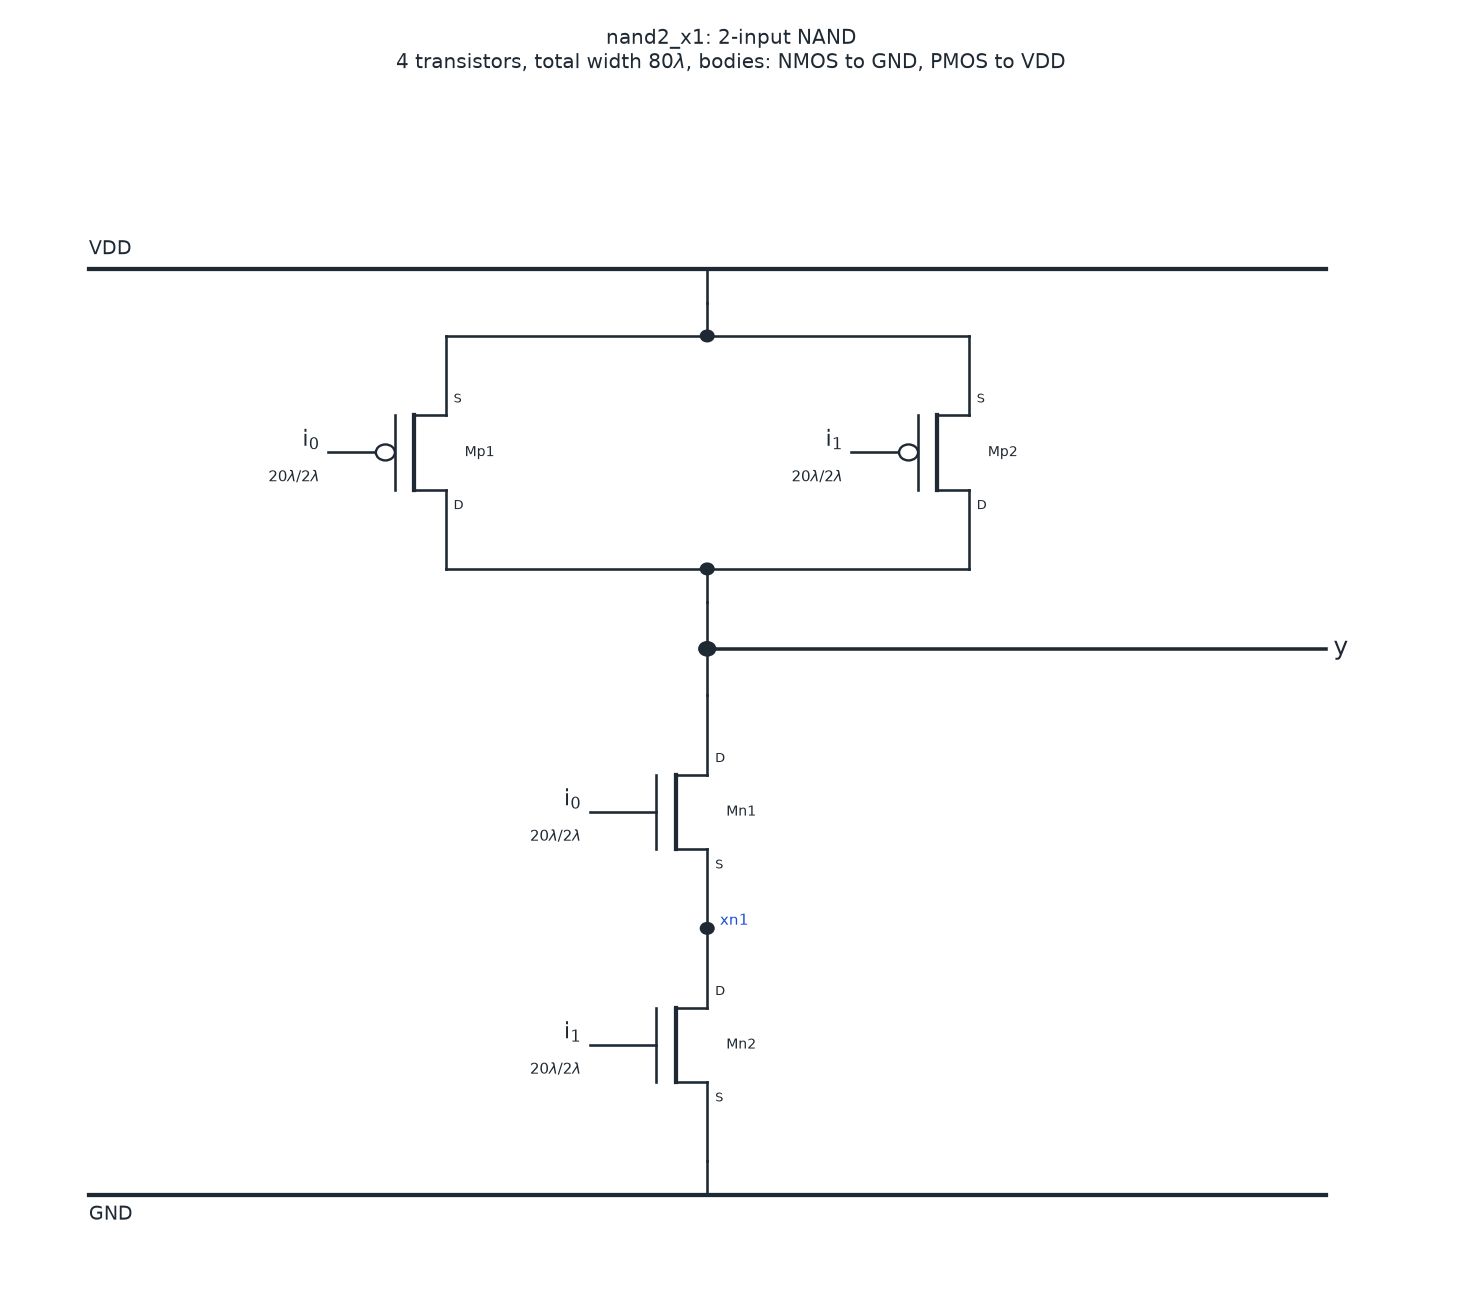
\includegraphics[width=0.32\textwidth]{figures/2.0d_gate-nand2.png}\hfill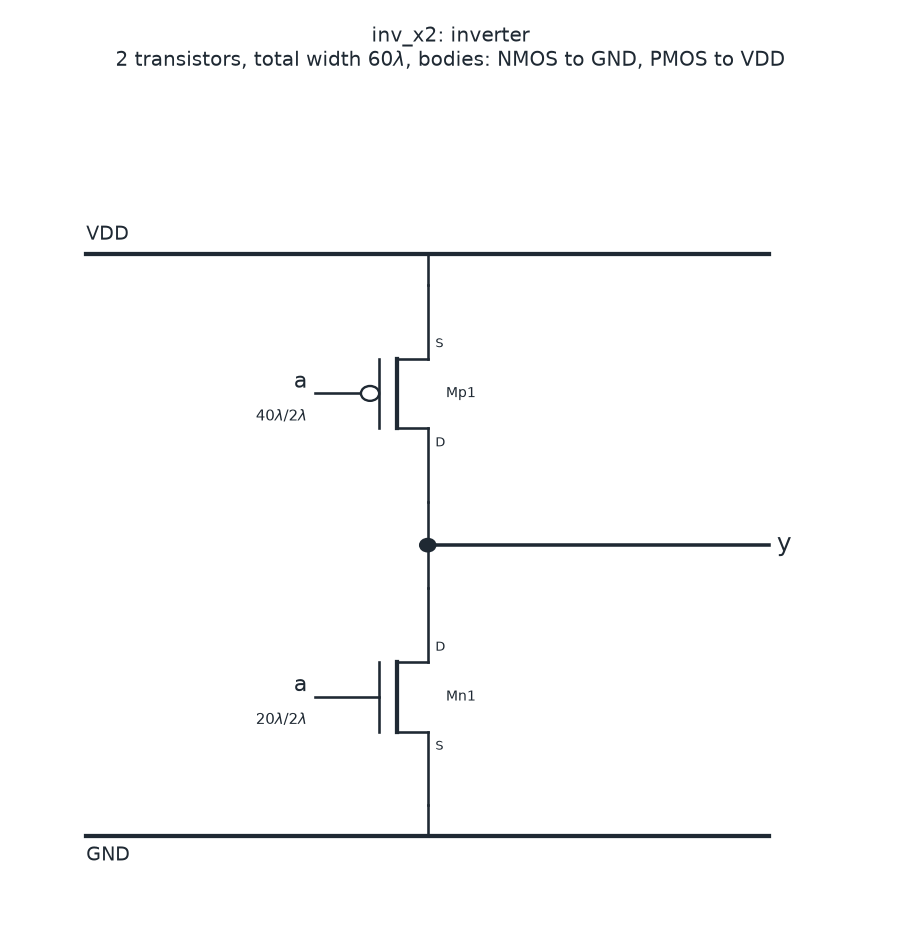
\includegraphics[width=0.32\textwidth]{figures/2.0e_gate-inv-x2.png}\caption{Transistor-level schematics: mode inverter, NAND2 on the carry path, output inverter.}\end{figure}

\textbf{Sizing.} The NAND2 and the output inverter were swept on the schematic of the full SIMD adder in mode 0, measuring the worst delay from Cin to S7 on the vector A = FF, B = 00 (figure~\ref{fig:sweep}). The fastest was NAND2 x1 with an x2 output inverter, 696.59\,ps. A larger NAND2 is slower: it adds load to CLA0's carry-out, which is on the critical path.

\begin{figure}[H]\centering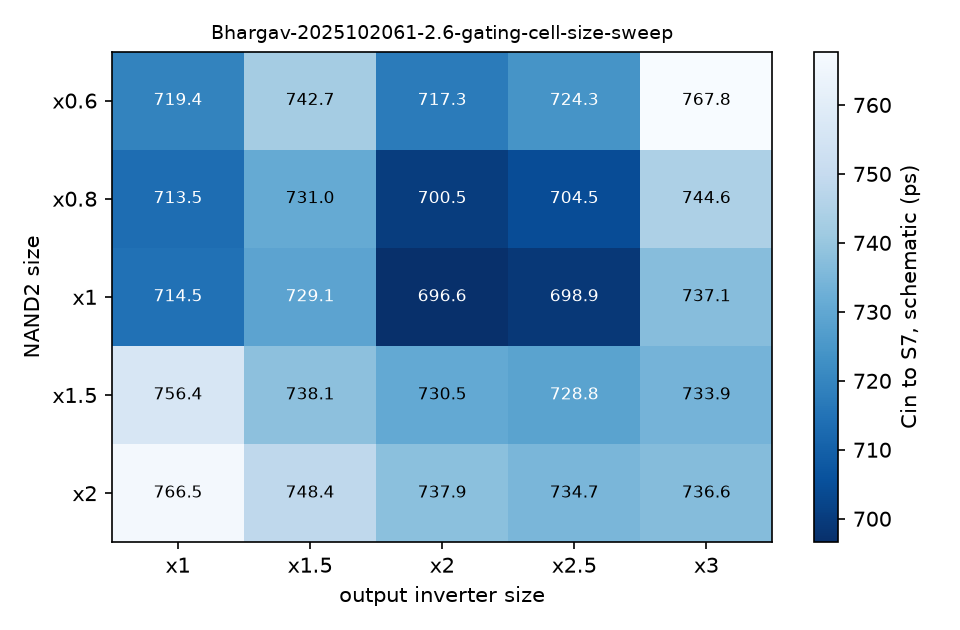
\includegraphics[width=0.7\textwidth]{figures/2.6_gating-cell-size-sweep.png}\caption{Gate sizing sweep: Cin to S7 in 8-bit mode, schematic.}\label{fig:sweep}\end{figure}

\begin{table}[H]\centering\small
\caption{Carry-gating cell on its own, cout\_lo to cin\_hi with a 20/10$\lambda$ load.}
\begin{tabular}{lrrr}
\toprule
\textbf{View} & \textbf{Worst (ps)} & \textbf{Output rising (ps)} & \textbf{Output falling (ps)} \\
\midrule
Schematic & 104.27 & 89.12 & 104.27 \\
Post-layout & 110.46 & 95.20 & 110.46 \\
\bottomrule
\end{tabular}
\end{table}

\begin{figure}[H]\centering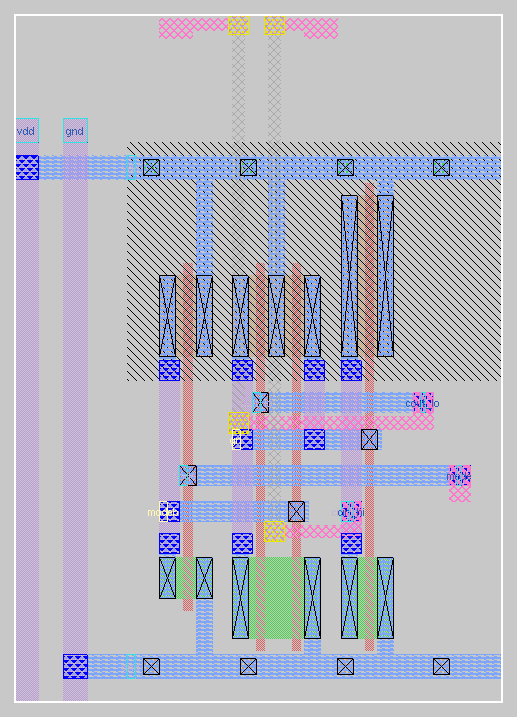
\includegraphics[width=0.55\textwidth]{figures/magic_gate.png}\caption{Gating cell in MAGIC, with its carry pads above it, as placed in the SIMD adder. The cell alone is 93 x 133 $\lambda$, DRC 0, LVS match: 8 merged devices, 8 nets.}\end{figure}

\section{Layout}

The layout keeps the two adders as two placed copies of one cell, as the task describes.
\begin{enumerate}
\item \textbf{Adder cell.} The Part I adder is laid out again by the Part I flow, with two extra metal 3 pads above its top row for C4 and C0. They are routed inside the cell like any other pin of those nets, so the top level can land a via on plain metal 3. The cell is DRC 0, LVS match: 194 merged devices, 108 nets, 3083.1\,$\mu$m$^2$.
\item \textbf{Gating cell.} Laid out by the same flow, with pads for cout\_lo and cin\_hi.
\item \textbf{Top level.} The adder cell is placed twice, with the gating cell between the copies in the SIMD design. The placement is flattened, then the inter-block carries are drawn on metal 5, which no cell uses. Port labels go on the cells' pin stubs, and the power straps join through buses below the cells.
\end{enumerate}
A first attempt placed all the gates of both adders in one set of rows. Its router ran out of tracks in the carry row, which led to the two-cell layout above.

The layout figures in this section are screenshots of MAGIC's own layout window.

\begin{figure}[H]\centering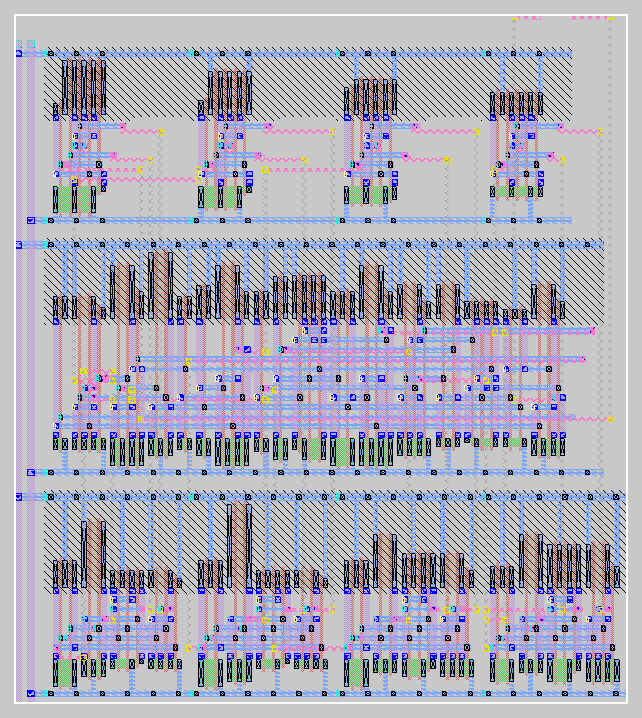
\includegraphics[width=\textwidth]{figures/magic_cla4_cell.png}\caption{The Part I adder cell in MAGIC, with the two extra carry pads above the sum row.}\end{figure}

\begin{figure}[H]\centering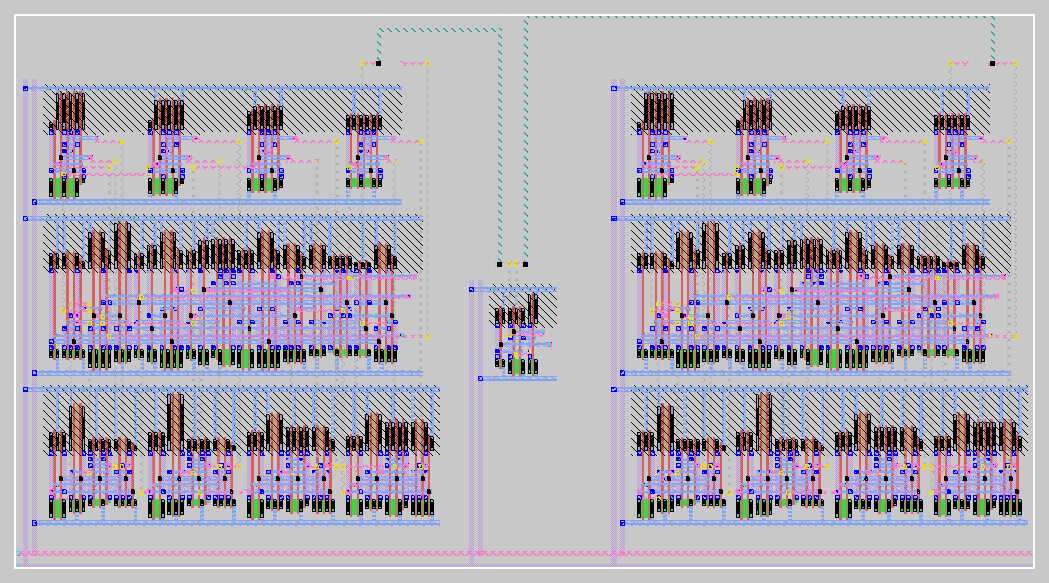
\includegraphics[width=\textwidth]{figures/magic_simd8.png}\caption{SIMD 8-bit adder in MAGIC: CLA0 on the left, the gating cell in the middle, CLA1 on the right. The dashed lines above are metal 5, carrying c4lo and cinh.}\end{figure}

\begin{figure}[H]\centering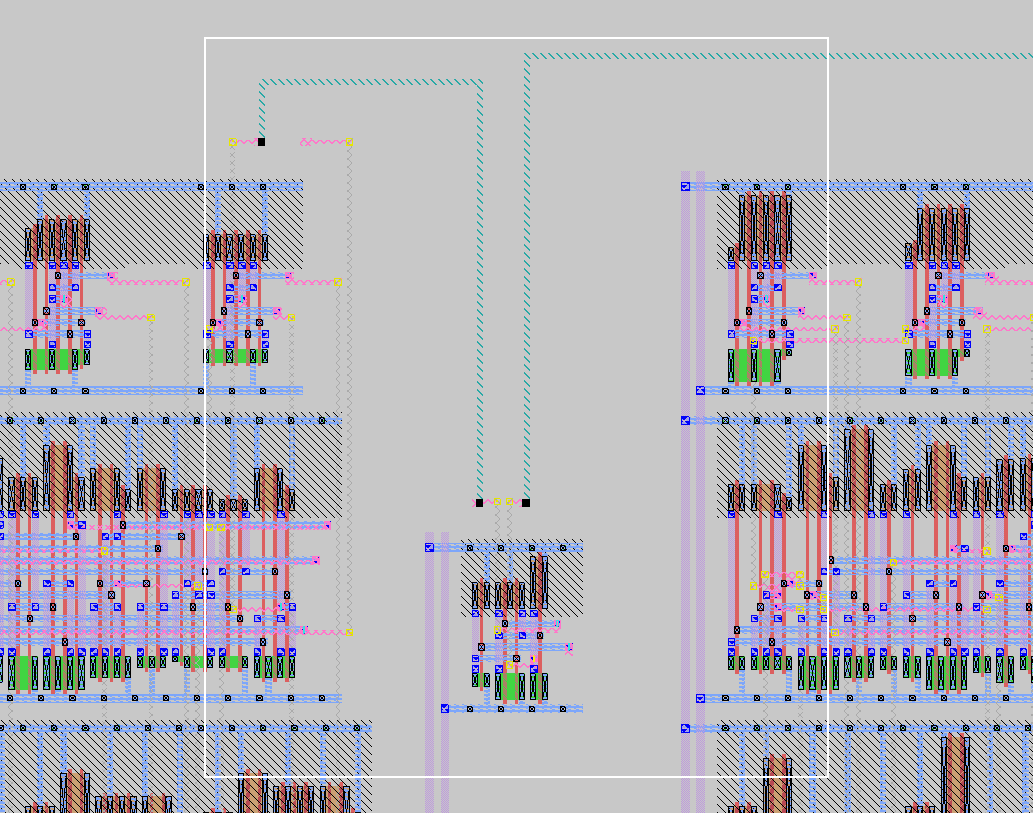
\includegraphics[width=0.85\textwidth]{figures/magic_simd8_gate_zoom.png}\caption{Close-up in MAGIC: the gating cell between CLA0 and CLA1 and its two metal 5 carries. The white rectangle is MAGIC's box, used to set the zoom.}\end{figure}

\begin{figure}[H]\centering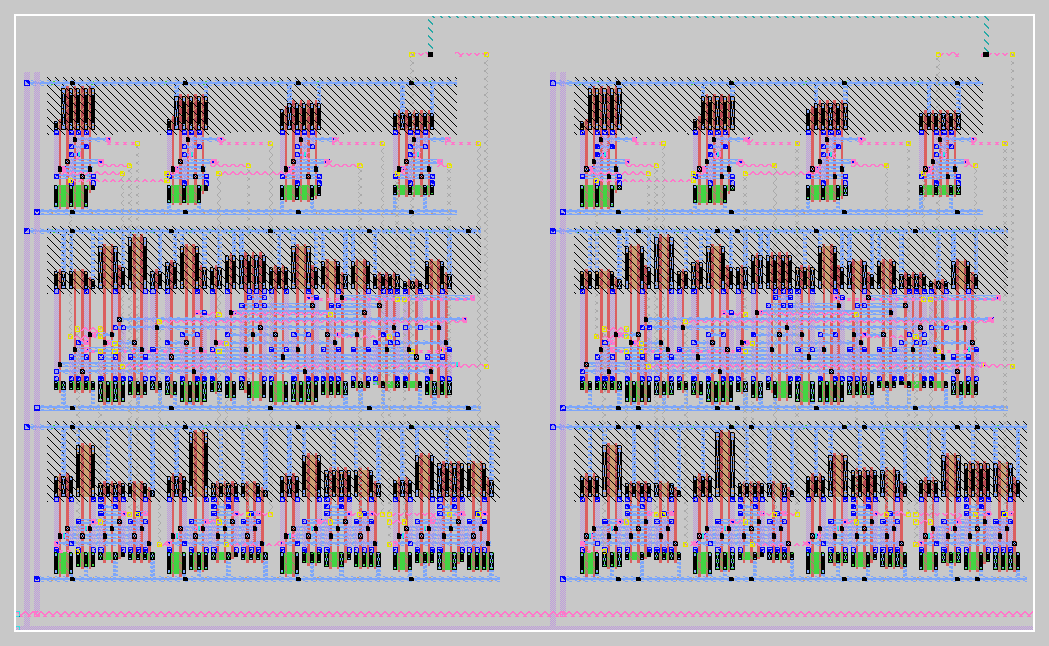
\includegraphics[width=\textwidth]{figures/magic_base8.png}\caption{Baseline 8-bit adder in MAGIC: c4lo runs on metal 5 straight from CLA0 to CLA1.}\end{figure}

\begin{table}[H]\centering\small
\caption{Layout checks and size.}
\resizebox{\textwidth}{!}{
\begin{tabular}{lrrrrrr}
\toprule
\textbf{Design} & \textbf{DRC} & \textbf{LVS} & \textbf{Transistors} & \textbf{Size ($\lambda$)} & \textbf{Area ($\mu$m$^2$)} & \textbf{Wire C (fF)} \\
\midrule
Baseline & 0 & match: 388 merged devices, 213 nets & 388 & 1236 x 774 & 7749.0 & 766.5 \\
SIMD & 0 & match: 396 merged devices, 218 nets & 396 & 1413 x 774 & 8858.7 & 792.4 \\
\bottomrule
\end{tabular}
}
\end{table}

The SIMD layout is 14.3\% larger. Most of that is the gating cell's slot between the two adders, not the 8 transistors themselves. LVS uses the project's own comparison script, as in Part I, because netgen was not available.

\section{Worst-case propagation delay in both modes}

An exhaustive search over all transitions of 17 or 18 inputs is too long, so the search is guided. Each case runs 13,312 single-input transitions in four Eulerian walks:
\begin{itemize}
\item every transition of CLA0's nine inputs, with CLA1 set to pass a carry through all four bits: A$_{hi}$ = F, B$_{hi}$ = 0, then A$_{hi}$ = 0, B$_{hi}$ = F;
\item every transition of CLA1's eight inputs, with CLA0's carry-out held at 0 and then at 1.
\end{itemize}
These walks contain every path from a CLA0 input across the block boundary to the upper sums and C8. Delay runs from the adder pin to the last 50\% crossing of the output, so false sums do not shorten it. Every output was also checked after each transition.

\begin{table}[H]\centering\small
\caption{Worst-case delay. tpd,pin is from the adder pin; tpd,drv includes the input driver.}
\resizebox{\textwidth}{!}{
\begin{tabular}{llrrrrl}
\toprule
\textbf{Case} & \textbf{View} & \textbf{Transitions} & \textbf{Errors} & \textbf{tpd,pin (ps)} & \textbf{tpd,drv (ps)} & \textbf{Worst arc} \\
\midrule
Baseline & schematic & 13312 & 0 & 855.22 & 934.52 & a3 rise to s5 fall, A=F7 B=04 C0=0 \\
Baseline & post-layout & 13312 & 0 & 1030.86 & 1115.70 & a3 rise to s5 fall, A=F7 B=04 C0=0 \\
SIMD, mode 0 & schematic & 13312 & 0 & 920.09 & 991.01 & a3 fall to s5 rise, A=FD B=07 C0=1 M=0 \\
SIMD, mode 0 & post-layout & 13312 & 0 & 1109.77 & 1183.87 & a3 fall to s5 rise, A=FF B=07 C0=1 M=0 \\
SIMD, mode 1 & schematic & 13312 & 0 & 516.31 & 590.23 & a5 rise to s7 rise, A=1F B=51 C0=0 M=1 \\
SIMD, mode 1 & post-layout & 13312 & 0 & 570.22 & 649.82 & a1 rise to s3 rise, A=F5 B=01 C0=0 M=1 \\
\bottomrule
\end{tabular}
}
\end{table}

\begin{figure}[H]\centering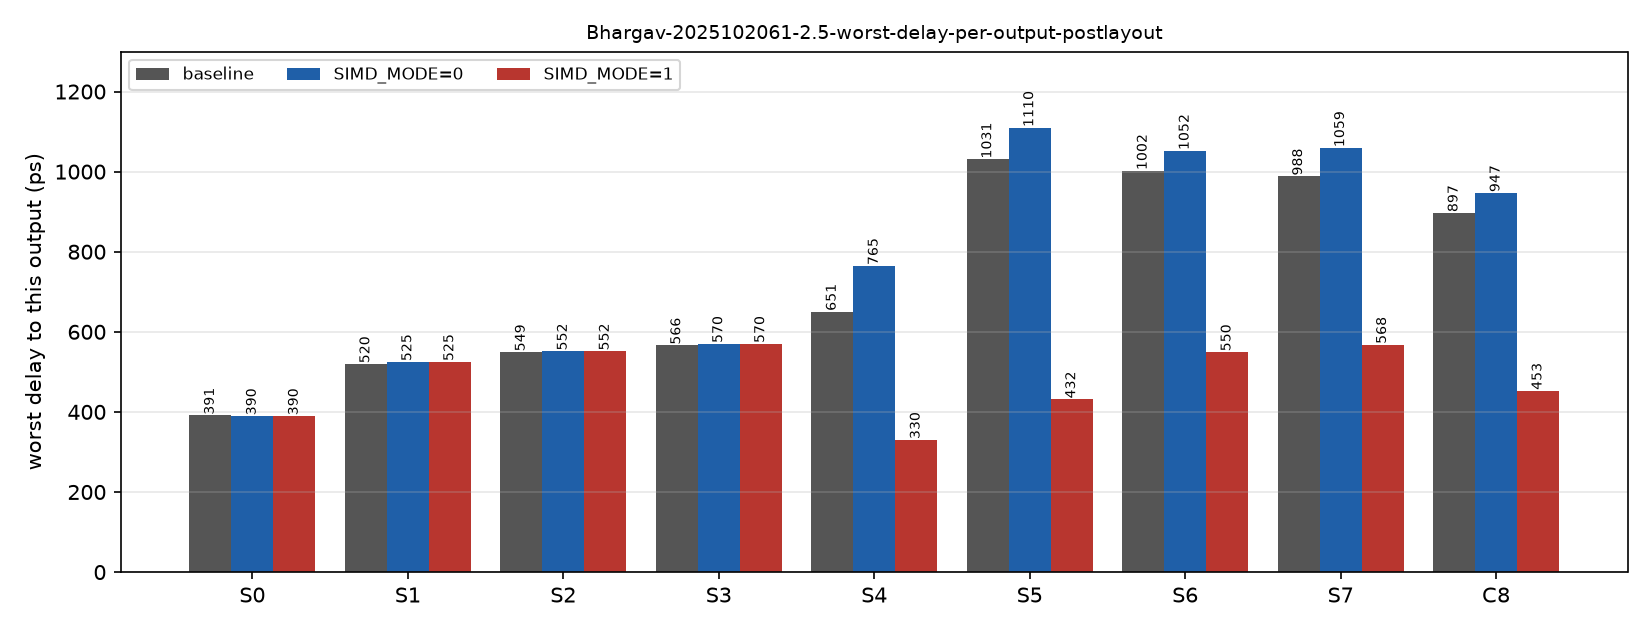
\includegraphics[width=\textwidth]{figures/2.5_worst-delay-per-output-postlayout.png}\caption{Worst post-layout delay to each output.}\end{figure}

\textbf{Reading the results.}
\begin{itemize}
\item In 8-bit mode the worst path runs from a3, through CLA0's carry tree and the inter-block carry, into CLA1's sums. The gating cell adds 78.91\,ps (7.65\%) to tpd,max post-layout, and 64.87\,ps (7.59\%) on the schematic.
\item In dual mode the carry never crosses, so the worst path stays inside one 4-bit block: 570.22\,ps post-layout. This is close to Part I's 579.88\,ps; the adder cell here was laid out again with the carry pads, and has the extra c4lo load.
\end{itemize}

\section{Delay penalty of the gating cell}

Worst-case carry propagation vector, A = 0xFF, B = 0x00, Cin$_0$ toggling. Delay from Cin$_0$ to S7, in mode 0 for the SIMD adder:

\[ \text{Delay penalty (\%)} = \frac{t_{pd,SIMD} - t_{pd,baseline}}{t_{pd,baseline}} \times 100\% \]

\begin{table}[H]\centering\small
\caption{Cin to S7 on the worst-case vector. In mode 1, S7 and C8 do not change.}
\resizebox{\textwidth}{!}{
\begin{tabular}{llrrrr}
\toprule
\textbf{View} & \textbf{Case} & \textbf{Cin rise to S7} & \textbf{Cin fall to S7} & \textbf{Cin rise to C8} & \textbf{Cin rise to c4lo} \\
\midrule
schematic & Baseline & 633.33 & 600.29 & 536.20 & -- \\
schematic & SIMD, mode 0 & 691.62 & 696.59 & 596.53 & 247.16 \\
schematic & SIMD, mode 1 & -- & -- & -- & 244.04 \\
post-layout & Baseline & 816.11 & 789.50 & 727.12 & -- \\
post-layout & SIMD, mode 0 & 877.83 & 903.93 & 781.59 & 323.84 \\
post-layout & SIMD, mode 1 & -- & -- & -- & 320.46 \\
\bottomrule
\end{tabular}
}
\end{table}

\begin{table}[H]\centering\small
\caption{Delay penalty, SIMD mode 0 against the baseline.}
\begin{tabular}{lrr}
\toprule
\textbf{View} & \textbf{Cin rise to S7} & \textbf{Cin fall to S7} \\
\midrule
Schematic & +58.28 ps, 9.20\% & +96.30 ps, 16.04\% \\
Post-layout & +61.72 ps, 7.56\% & +114.44 ps, 14.49\% \\
\bottomrule
\end{tabular}
\end{table}

\begin{figure}[H]\centering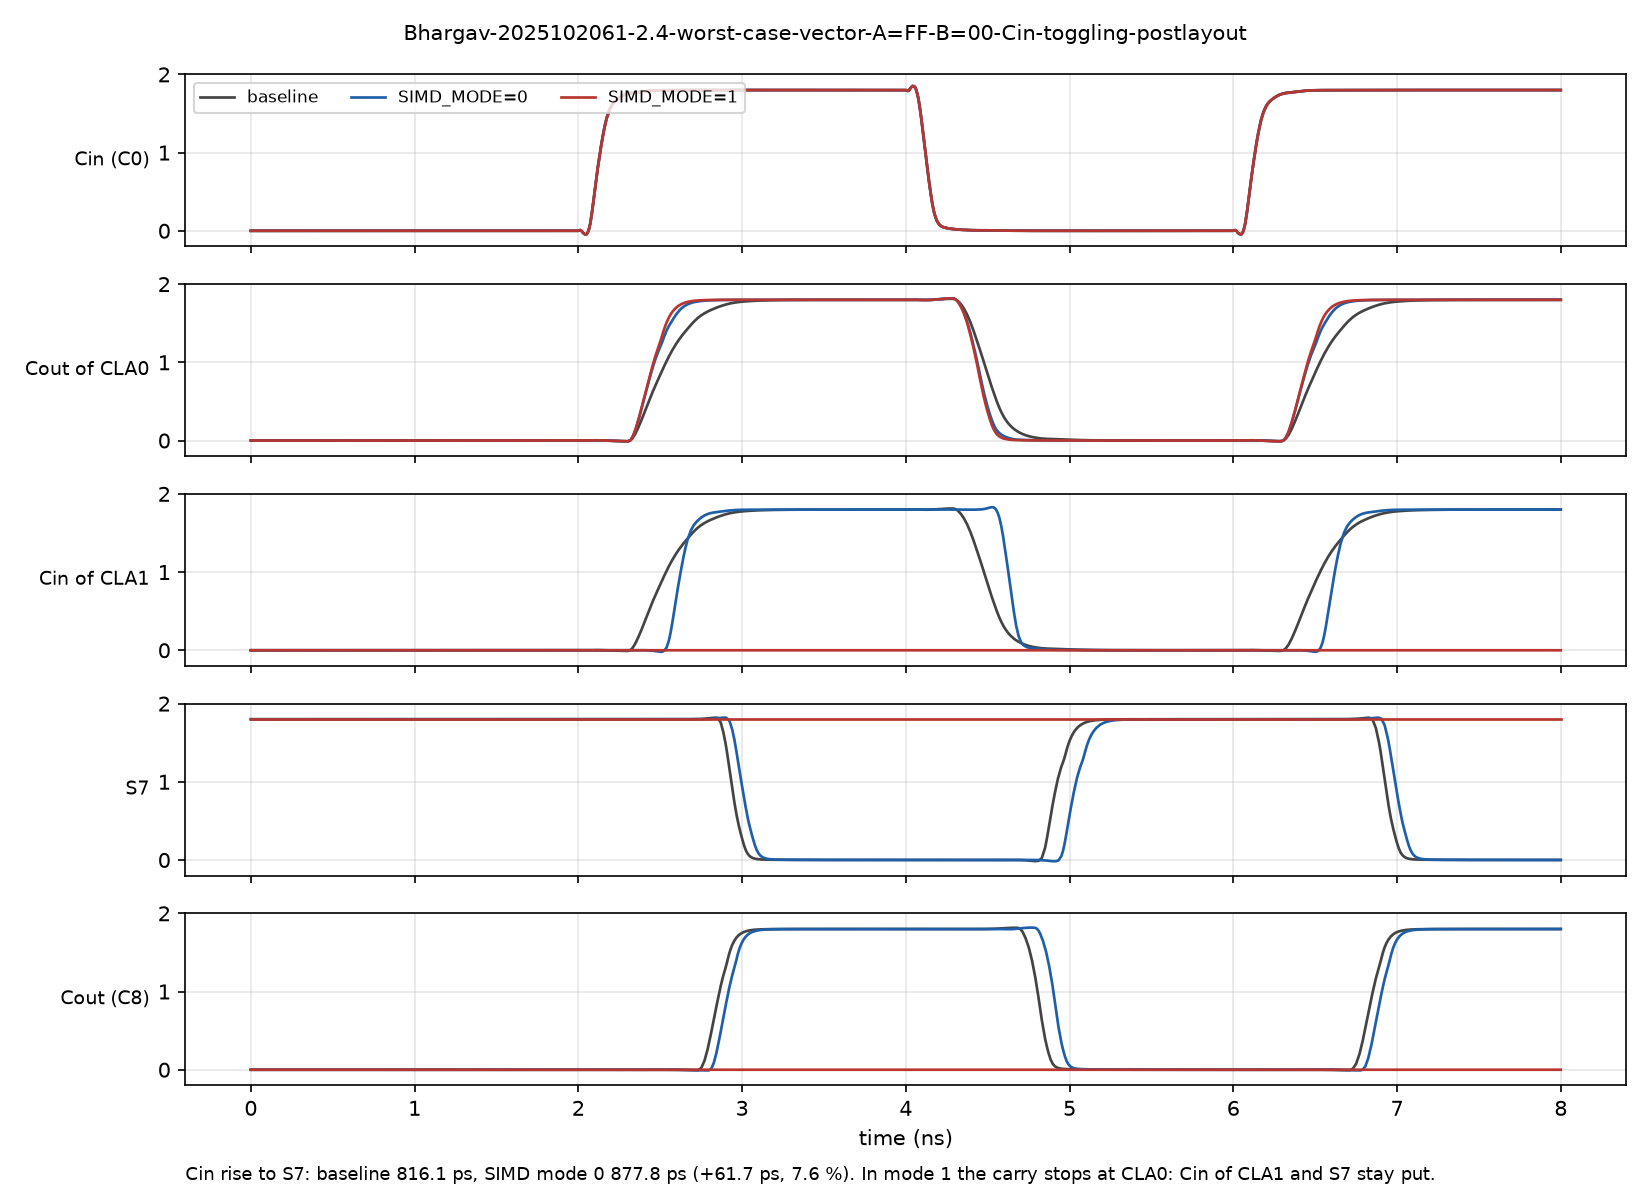
\includegraphics[width=\textwidth]{figures/2.4_worst-case-vector-postlayout.png}\caption{Post-layout waveforms on the worst-case vector, all three cases.}\label{fig:waves}\end{figure}

\textbf{Why the penalty is smaller than the gate's own delay.} The gate alone takes 110.46\,ps, but the rising-edge penalty is only 61.72\,ps. In the baseline, CLA0's carry-out drives CLA1's carry-in load directly. In the SIMD design it drives only the NAND2 input and the output load, so it switches sooner, which figure~\ref{fig:waves} shows. On the falling edge the penalty is larger, 114.44\,ps.

\section{Maximum frequency and power penalty}

The maximum frequency uses the course formula, $f_{max} = 1 / (t_{pd,max} + t_{setup} + t_{hold})$, with the Part I flip-flop's post-layout $t_{setup} = 38.0$\,ps and $t_{hold} = 45.7$\,ps.

\begin{table}[H]\centering\small
\caption{Course-formula maximum frequency, post-layout.}
\begin{tabular}{lrrr}
\toprule
\textbf{Case} & \textbf{tpd,max (ps)} & \textbf{Period (ps)} & \textbf{fmax (GHz)} \\
\midrule
Baseline & 1030.86 & 1114.56 & 0.897 \\
SIMD, mode 0 & 1109.77 & 1193.47 & 0.838 \\
SIMD, mode 1 & 570.22 & 653.92 & 1.529 \\
\bottomrule
\end{tabular}
\end{table}

\textbf{The formula's clock is too short for some inputs.} At each design's own course-formula clock, random vectors gave wrong outputs at the end of some cycles: 10 of 200 for the baseline and 46 for SIMD mode 0. These vectors change several inputs at once, which is slower than the single-input worst case the search found, as in Part I. Power measured while outputs fail is not trustworthy. So the shortest clock at which all three cases settle on the same 200 random vectors was found:

\begin{table}[H]\centering\small
\caption{Wrong output samples on 200 random vectors, post-layout.}
\begin{tabular}{lrrr}
\toprule
\textbf{Period (ps)} & \textbf{Baseline} & \textbf{SIMD, mode 0} & \textbf{SIMD, mode 1} \\
\midrule
1250 & 6 & 17 & 0 \\
1300 & 2 & 5 & 0 \\
1350 & 0 & 2 & 0 \\
1400 & 0 & 0 & 0 \\
1500 & 0 & 0 & 0 \\
\bottomrule
\end{tabular}
\end{table}

All three cases settle at 1400\,ps, so power is compared there. All three get identical input vectors: 10 cycles as the task asks, and 200 vectors as a check. Power is the adder's own supply only: drivers and load inverters use a separate source.

\[ \text{Power penalty (\%)} = \frac{P_{SIMD,\,mode\,0} - P_{baseline}}{P_{baseline}} \times 100\% \]

\begin{table}[H]\centering\small
\caption{Average power at 1400 ps, post-layout. 0 wrong outputs in every run.}
\begin{tabular}{lrr}
\toprule
\textbf{Case} & \textbf{10 cycles ($\mu$W)} & \textbf{200 vectors ($\mu$W)} \\
\midrule
Baseline & 1695.2 & 1876.3 \\
SIMD, mode 0 & 1720.7 & 1919.5 \\
SIMD, mode 1 & 1592.4 & 1713.7 \\
\bottomrule
\end{tabular}
\end{table}

\textbf{Power penalty in 8-bit mode:} 1.50\% over 10 cycles, and 2.30\% over 200 vectors. The gating cell adds little switching: 8 small transistors, with the mode inverter idle. Dual mode uses the least power, because a carry stopped at the boundary does not ripple through CLA1.

\section{Energy-delay product}

\[ EDP = P_{avg} \times t_{pd}^2 \]

\begin{table}[H]\centering\small
\caption{Energy-delay product, with the 10-cycle power at the common clock and the post-layout tpd,max.}
\begin{tabular}{lrrr}
\toprule
\textbf{Case} & \textbf{Pavg ($\mu$W)} & \textbf{tpd,max (ps)} & \textbf{EDP (J s)} \\
\midrule
Baseline & 1695.2 & 1030.86 & 1.801e-21 \\
SIMD, mode 0 & 1720.7 & 1109.77 & 2.119e-21 \\
SIMD, mode 1 & 1592.4 & 570.22 & 5.178e-22 \\
\bottomrule
\end{tabular}
\end{table}

In 8-bit mode the SIMD adder's EDP is 17.6\% higher than the baseline's. Delay counts twice in EDP, so the 7.7\% delay penalty dominates the 1.5\% power penalty. In dual mode the EDP is far lower, because each add is only 4 bits long.

\section{Summary and limits}

\begin{table}[H]\centering\small
\caption{Cost of reconfigurability: SIMD mode 0 against the baseline, post-layout.}
\begin{tabular}{lrrr}
\toprule
\textbf{Measure} & \textbf{Baseline} & \textbf{SIMD mode 0} & \textbf{Penalty} \\
\midrule
Cin rise to S7 (ps) & 816.11 & 877.83 & 7.56\% \\
tpd,max (ps) & 1030.86 & 1109.77 & 7.65\% \\
Power, 10 cycles ($\mu$W) & 1695.2 & 1720.7 & 1.50\% \\
EDP (J s) & 1.801e-21 & 2.119e-21 & 17.6\% \\
Transistors & 388 & 396 & +8 \\
Area ($\mu$m$^2$) & 7749.0 & 8858.7 & 14.3\% \\
\bottomrule
\end{tabular}
\end{table}

\begin{itemize}
\item \textbf{Guided search.} The worst-case search is guided and single-input; it is not exhaustive. Multi-input changes are slower, as the settle test shows, and their exact worst case was not searched.
\item \textbf{Power clock.} Power is compared at a common verified clock, not at each design's course-formula fmax, because at that clock some vectors fail.
\item \textbf{Area.} It is the bounding box, including gaps and routing channels.
\item \textbf{Wire resistance.} Not extracted, as in Part I: MAGIC's resistance extraction crashed.
\end{itemize}

\appendix\section{Netlists}

Generated from \texttt{part2/cells/simd.py}. The full files, with the Part I cells, are in \texttt{part2/schematics/}.

\subsection*{Carry-gating cell}\begin{small}\begin{verbatim}
.subckt carry_gate_n1_i2 cout_lo mode cin_hi vdd gnd
Xinvm mode modeb vdd gnd inv_x1
Xnandg cout_lo modeb gn vdd gnd nand2_x1
Xinvg gn cin_hi vdd gnd inv_x2
.ends carry_gate_n1_i2
\end{verbatim}\end{small}

\subsection*{SIMD 8-bit adder, top level}\begin{small}\begin{verbatim}
.subckt simd8 a0 a1 a2 a3 a4 a5 a6 a7 b0 b1 b2 b3 b4 b5 b6 b7 c0 mode s0 s1 s2 s3 s4 s5 s6
+ s7 c8 c4lo vdd gnd
Xcla0 a0 a1 a2 a3 b0 b1 b2 b3 c0 s0 s1 s2 s3 c4lo vdd gnd cla4_final
Xgate c4lo mode cinh vdd gnd carry_gate_n1_i2
Xcla1 a4 a5 a6 a7 b4 b5 b6 b7 cinh s4 s5 s6 s7 c8 vdd gnd cla4_final
.ends simd8
\end{verbatim}\end{small}

\subsection*{Baseline 8-bit adder, top level}\begin{small}\begin{verbatim}
.subckt base8 a0 a1 a2 a3 a4 a5 a6 a7 b0 b1 b2 b3 b4 b5 b6 b7 c0 s0 s1 s2 s3 s4 s5 s6 s7 c8
+ vdd gnd
Xcla0 a0 a1 a2 a3 b0 b1 b2 b3 c0 s0 s1 s2 s3 c4lo vdd gnd cla4_final
Xcla1 a4 a5 a6 a7 b4 b5 b6 b7 c4lo s4 s5 s6 s7 c8 vdd gnd cla4_final
.ends base8
\end{verbatim}\end{small}

\section{Reproducing the results}
From \texttt{part2/cells/}, in order: \texttt{simd.py gate}, \texttt{netlists}, \texttt{cells}, \texttt{layout\_h simd base}, \texttt{search} for each case and view, \texttt{penalty}, \texttt{settle}, \texttt{power 1400}, \texttt{waves}, \texttt{summary}, then \texttt{make\_report.py}.
\end{document}
